\documentclass[lualatex,aspectratio=169,12pt]{beamer}

% ===== Japanese support =====
\usepackage{luatexja}
\usepackage{luatexja-fontspec}

% ===== Packages =====
\usepackage{amsmath, amssymb, bm}
\usepackage{booktabs}
\usepackage{array}
\usepackage{tikz}
\usetikzlibrary{positioning, arrows.meta, shapes.geometric}
\usepackage{pgfplots}
\pgfplotsset{compat=1.18}
\usepackage{listings}

% ===== Theme =====
\usetheme{metropolis}
\usecolortheme{default}
\setbeamercolor{normal text}{fg=black!85}
\setbeamercolor{frametitle}{bg=blue!15!white, fg=blue!60!black}
\setbeamercolor{title separator}{fg=blue!60!black}
\setbeamercolor{progress bar}{fg=blue!60!black}
\setbeamercolor{block title}{bg=blue!15, fg=blue!60!black}
\setbeamercolor{block body}{bg=blue!5}
\setbeamercolor{alerted text}{fg=orange!80!black}

% ===== Listings =====
\lstset{
  language=R,
  basicstyle=\ttfamily\footnotesize,
  backgroundcolor=\color{gray!10},
  frame=single,
  breaklines=true,
  keywordstyle=\color{blue!70!black},
  commentstyle=\color{green!50!black},
}

% ===== Macros =====
\newcommand{\mvn}{\mathrm{MVN}}
\newcommand{\IW}{\mathrm{inverse\text{-}Wishart}}
\newcommand{\IG}{\mathrm{inverse\text{-}gamma}}
\newcommand{\tr}{\mathrm{tr}}

% ===== Title =====
\title{The Multivariate Normal Model}
\subtitle{Hoff 第7章 ― 多変量正規モデルのベイズ推論}
\author{}
\date{}
\institute{}

\begin{document}

\maketitle

% ----------------------------------------
\begin{frame}{目次}
  \setbeamertemplate{section in toc}[sections numbered]
  \tableofcontents
\end{frame}

% ==========================================
\section{7.1 多変量正規分布}
% ==========================================

\begin{frame}{なぜ多変量正規分布か？}
  第5・6章：1変数 $y \in \mathbb{R}$ → 正規分布

  \bigskip
  現実のデータは\alert{複数の変数}を同時に持つ：
  \begin{itemize}
    \item 血圧・体重・年齢
    \item 読解テストの時間1・時間2のスコア
    \item 遺伝子発現量の複数遺伝子
  \end{itemize}

  \bigskip
  \begin{block}{第7章のテーマ}
    正規分布のベイズ推論を\textbf{ベクトル}に拡張する
  \end{block}

  \vspace{0.3em}
  \begin{center}
  \begin{tabular}{c@{\quad$\to$\quad}c}
    平均 $\theta$ & 平均ベクトル $\bm{\theta}$ \\
    分散 $\sigma^2$ & 共分散行列 $\Sigma$ \\
    inverse-gamma & inverse-\textbf{Wishart} \\
  \end{tabular}
  \end{center}
\end{frame}

\begin{frame}{多変量正規分布の定義}
  \begin{block}{定義：$\bm{Y} \sim \mvn(\bm{\theta}, \Sigma)$}
    $p$ 次元確率ベクトル $\bm{Y}$ の密度：
    \[
      p(\bm{y} \mid \bm{\theta}, \Sigma)
      = (2\pi)^{-p/2}|\Sigma|^{-1/2}
        \exp\!\left\{-\frac{1}{2}(\bm{y}-\bm{\theta})^\top\Sigma^{-1}(\bm{y}-\bm{\theta})\right\}
    \]
  \end{block}

  \begin{itemize}
    \item $\bm{\theta}$：\textbf{平均ベクトル}（$p$ 次元）
    \item $\Sigma$：$p\times p$ \textbf{共分散行列}（対称・正定値）
    \item $(\bm{y}-\bm{\theta})^\top\Sigma^{-1}(\bm{y}-\bm{\theta})$：\textbf{マハラノビス距離の2乗}
  \end{itemize}

  \medskip
  \textbf{1次元との対応：}$p=1$ のとき $\Sigma=\sigma^2$ → 通常の正規分布に帰着
\end{frame}

\begin{frame}{等高線は楕円}
  \[
    \{y : (\bm{y}-\bm{\theta})^\top\Sigma^{-1}(\bm{y}-\bm{\theta}) = c\} \text{ → 楕円}
  \]

  \vspace{-0.5em}
  \begin{center}
  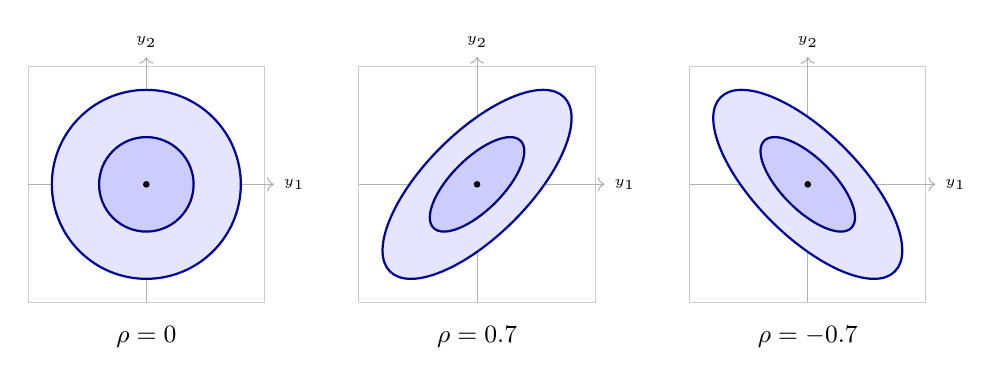
\begin{tikzpicture}[scale=0.6]
    \foreach \r/\x/\lab in {0/0/{$\rho=0$}, 0.7/7/{$\rho=0.7$}, -0.7/14/{$\rho=-0.7$}} {
      \begin{scope}[xshift=\x cm]
        \draw[gray!40] (-2.5,-2.5) rectangle (2.5,2.5);
        \draw[gray!60,->] (-2.5,0)--(2.7,0) node[right,black]{\tiny $y_1$};
        \draw[gray!60,->] (0,-2.5)--(0,2.7) node[above,black]{\tiny $y_2$};
        \pgfmathsetmacro{\a}{sqrt(1+\r)}
        \pgfmathsetmacro{\b}{sqrt(1-\r)}
        \fill[blue!10,rotate=45] (0,0) ellipse ({2*\a} and {2*\b});
        \draw[blue!60!black,thick,rotate=45] (0,0) ellipse ({2*\a} and {2*\b});
        \fill[blue!20,rotate=45] (0,0) ellipse ({\a} and {\b});
        \draw[blue!50!black,thick,rotate=45] (0,0) ellipse ({\a} and {\b});
        \fill (0,0) circle (2pt);
        \node[below] at (0,-2.8) {\small \lab};
      \end{scope}
    }
  \end{tikzpicture}
  \end{center}

  \begin{itemize}
    \item $\rho = 0$：円（変数間に相関なし）
    \item $\rho > 0$：右上がり楕円（正の相関）
    \item $\rho < 0$：右下がり楕円（負の相関）
  \end{itemize}
\end{frame}

\begin{frame}{1次元との比較表}
  \begin{center}
  \renewcommand{\arraystretch}{1.5}
  \begin{tabular}{lll}
  \toprule
   & 正規分布 & 多変量正規分布 \\
  \midrule
  データ & $y \in \mathbb{R}$ & $\bm{y} \in \mathbb{R}^p$ \\
  中心 & 平均 $\theta$ & 平均ベクトル $\bm{\theta}$ \\
  広がり & 分散 $\sigma^2$ & 共分散行列 $\Sigma$ \\
  精度 & $1/\sigma^2$ & 精度行列 $\Sigma^{-1}$ \\
  距離 & $(y-\theta)^2/\sigma^2$ & $(\bm{y}-\bm{\theta})^\top\Sigma^{-1}(\bm{y}-\bm{\theta})$ \\
  標本平均 & $\bar{Y} \sim N(\theta,\sigma^2/n)$ & $\bar{\bm{Y}} \sim \mvn(\bm{\theta},\Sigma/n)$ \\
  \bottomrule
  \end{tabular}
  \end{center}
\end{frame}

% ==========================================
\section{7.2 平均ベクトルの半共役事前分布}
% ==========================================

\begin{frame}{モデル設定}
  \begin{block}{階層モデル}
    \begin{align*}
      \bm{Y}_1, \ldots, \bm{Y}_n \mid \bm{\theta}, \Sigma
      &\;\overset{\mathrm{i.i.d.}}{\sim}\; \mvn(\bm{\theta}, \Sigma) \quad \text{（尤度）}\\
      \bm{\theta}
      &\;\sim\; \mvn(\bm{\mu}_0, \Lambda_0) \quad\quad\quad \text{（事前分布）}
    \end{align*}
  \end{block}

  \bigskip
  \begin{itemize}
    \item $\Sigma$：この節では\textbf{既知}として扱う（7.3節で未知に拡張）
    \item \alert{「半共役」}：$\bm{\theta}$ の事前分布は $\Sigma$ を条件に共役だが，
          $(\bm{\theta}, \Sigma)$ の同時分布としては共役でない
  \end{itemize}
\end{frame}

\begin{frame}{事後分布の導出（概要）}
  \[
    p(\bm{\theta} \mid \bm{Y}, \Sigma)
    \propto \underbrace{p(\bm{Y}\mid\bm{\theta},\Sigma)}_{\text{尤度}}
            \cdot\underbrace{p(\bm{\theta})}_{\text{事前}}
  \]

  \bigskip
  指数の中をまとめると（$\bm{\theta}$ に関して）：
  \[
    -\frac{1}{2}\left[\bm{\theta}^\top\underbrace{\left(\Lambda_0^{-1} + n\Sigma^{-1}\right)}_{=\, \Lambda_n^{-1}}\bm{\theta}
    - 2\underbrace{\left(\Lambda_0^{-1}\bm{\mu}_0 + n\Sigma^{-1}\bar{\bm{y}}\right)^\top}_{=\,\bm{\mu}_n^\top\Lambda_n^{-1}}\bm{\theta}\right]
  \]

  \medskip
  これは $\mvn(\bm{\mu}_n, \Lambda_n)$ の\textbf{核（kernel）}
\end{frame}

\begin{frame}{事後分布の結果}
  \begin{block}{定理：$\bm{\theta}$ の事後分布}
    \[
      \bm{\theta} \mid \bm{Y}, \Sigma \;\sim\; \mvn(\bm{\mu}_n, \Lambda_n)
    \]
    \begin{align*}
      \Lambda_n &= \left(\Lambda_0^{-1} + n\Sigma^{-1}\right)^{-1} \\[4pt]
      \bm{\mu}_n &= \Lambda_n\left(\Lambda_0^{-1}\bm{\mu}_0 + n\Sigma^{-1}\bar{\bm{y}}\right)
    \end{align*}
  \end{block}

  \vspace{0.5em}
  \begin{center}
  \begin{tabular}{r@{\;=\;}l@{\;+\;}l}
    \multicolumn{3}{c}{\textbf{精度行列の加算}}\\[2pt]
    $\Lambda_n^{-1}$ & $\Lambda_0^{-1}$ & $n\Sigma^{-1}$ \\
    （事後の精度） & （事前の精度） & （データの精度）
  \end{tabular}
  \end{center}
\end{frame}

\begin{frame}{1次元との完全な対応}
  \begin{center}
  \renewcommand{\arraystretch}{1.8}
  \begin{tabular}{lll}
  \toprule
   & 1次元（5.2節） & 多変量（7.2節） \\
  \midrule
  精度の加算 & $\dfrac{1}{\tau_n^2} = \dfrac{1}{\tau_0^2} + \dfrac{n}{\sigma^2}$ &
              $\Lambda_n^{-1} = \Lambda_0^{-1} + n\Sigma^{-1}$ \\[6pt]
  事後平均 & $\mu_n = \tau_n^2\!\left(\dfrac{\mu_0}{\tau_0^2} + \dfrac{n\bar{y}}{\sigma^2}\right)$ &
             $\bm{\mu}_n = \Lambda_n\!\left(\Lambda_0^{-1}\bm{\mu}_0 + n\Sigma^{-1}\bar{\bm{y}}\right)$ \\[6pt]
  事後分布 & $\theta \sim N(\mu_n, \tau_n^2)$ & $\bm{\theta} \sim \mvn(\bm{\mu}_n, \Lambda_n)$ \\
  \bottomrule
  \end{tabular}
  \end{center}

  \vspace{0.5em}
  \centering
  \alert{スカラー → 行列 に置き換えるだけ}
\end{frame}

% ==========================================
\section{7.3 逆ウィシャート分布}
% ==========================================

\begin{frame}{逆ウィシャート分布とは}
  \begin{block}{定義：$\Sigma \sim \IW(\nu_0, S_0^{-1})$}
    \[
      p(\Sigma) \propto |\Sigma|^{-(\nu_0+p+1)/2}\exp\!\left\{-\frac12\tr(S_0\Sigma^{-1})\right\}
    \]
    \begin{itemize}
      \item $\nu_0 > p-1$：自由度
      \item $S_0$：スケール行列（$p\times p$ 正定値）
      \item $E[\Sigma] = \dfrac{S_0}{\nu_0 - p - 1}$（$\nu_0 > p+1$）
    \end{itemize}
  \end{block}

  \bigskip
  \begin{center}
  \textbf{逆ガンマ（1次元）→ 逆ウィシャート（多次元）}
  \end{center}
\end{frame}

\begin{frame}{1次元との対応表}
  \begin{center}
  \renewcommand{\arraystretch}{1.6}
  \begin{tabular}{lll}
  \toprule
   & 1次元正規モデル & 多変量正規モデル \\
  \midrule
  推定する広がり & 分散 $\sigma^2 > 0$ & 共分散行列 $\Sigma$（正定値）\\
  共役事前分布 & $\IG(\nu_0/2, \nu_0\sigma_0^2/2)$ & $\IW(\nu_0, S_0^{-1})$ \\
  指数の中 & $-\nu_0\sigma_0^2/(2\sigma^2)$ & $-\frac12\tr(S_0\Sigma^{-1})$ \\
  べき乗 & $(\sigma^2)^{-(\nu_0/2+1)}$ & $|\Sigma|^{-(\nu_0+p+1)/2}$ \\
  更新 & 平方和 $\sum(y_i-\theta)^2$ を足す & 平方和行列 $S_\theta$ を足す \\
  \bottomrule
  \end{tabular}
  \end{center}
\end{frame}

\begin{frame}{トレース恒等式：なぜ $\tr$ が出るか}
  \textbf{スカラー：}$a^\top B a = \tr(Baa^\top)$（スカラーのトレースは自身）

  \bigskip
  この恒等式を使うと：
  \begin{align*}
    \sum_{i=1}^n (\bm{y}_i-\bm{\theta})^\top\Sigma^{-1}(\bm{y}_i-\bm{\theta})
    &= \sum_{i=1}^n \tr\!\left(\Sigma^{-1}(\bm{y}_i-\bm{\theta})(\bm{y}_i-\bm{\theta})^\top\right) \\
    &= \tr\!\left(\Sigma^{-1}\underbrace{\sum_{i=1}^n(\bm{y}_i-\bm{\theta})(\bm{y}_i-\bm{\theta})^\top}_{S_\theta}\right) \\
    &= \tr(S_\theta\Sigma^{-1})
  \end{align*}

  \vspace{0.3em}
  $S_\theta = \sum_i(\bm{y}_i-\bm{\theta})(\bm{y}_i-\bm{\theta})^\top$：\alert{平方和行列}（$p\times p$）
\end{frame}

\begin{frame}{$\Sigma$ の条件付き事後分布}
  $\bm{\theta}$ を条件としたとき：

  \bigskip
  \begin{tabular}{rl}
    尤度 $\propto$ & $|\Sigma|^{-n/2}\exp\{-\frac12\tr(S_\theta\Sigma^{-1})\}$ \\[4pt]
    事前 $\propto$ & $|\Sigma|^{-(\nu_0+p+1)/2}\exp\{-\frac12\tr(S_0\Sigma^{-1})\}$ \\
  \end{tabular}

  \bigskip
  掛け合わせると
  \[
    p(\Sigma\mid\bm{Y},\bm{\theta})
    \propto |\Sigma|^{-(\nu_0+n+p+1)/2}\exp\!\left\{-\frac12\tr\!\left((S_0+S_\theta)\Sigma^{-1}\right)\right\}
  \]

  \begin{block}{定理：$\Sigma$ の条件付き事後分布}
    \[
      \Sigma \mid \bm{Y}, \bm{\theta}
      \;\sim\; \IW\!\left(\nu_0+n,\; (S_0 + S_\theta)^{-1}\right)
    \]
  \end{block}
\end{frame}

\begin{frame}{更新則の直感}
  \begin{center}
  \renewcommand{\arraystretch}{1.8}
  \begin{tabular}{ccc}
  \toprule
  更新前 & & 更新後 \\
  \midrule
  自由度 $\nu_0$ & $+ n$ & $\nu_0 + n$ \\
  スケール行列 $S_0$ & $+ S_\theta$ & $S_0 + S_\theta$ \\
  \bottomrule
  \end{tabular}
  \end{center}

  \bigskip
  \begin{itemize}
    \item $\nu_0$：事前の「仮想サンプル数」
    \item $S_0$：事前の「仮想平方和行列」
    \item $S_\theta = \sum(\bm{y}_i-\bm{\theta})(\bm{y}_i-\bm{\theta})^\top$：データの平方和行列
  \end{itemize}
\end{frame}

% ==========================================
\section{7.4 ギブスサンプラー}
% ==========================================

\begin{frame}{なぜ MCMC が必要か}
  \textbf{問題：}$(\bm{\theta}, \Sigma)$ の\textbf{同時}事後分布は解析的に求められない

  \bigskip
  しかし\textbf{条件付き}事後分布は両方とも既知：
  \begin{align*}
    \bm{\theta} \mid \bm{Y}, \Sigma &\;\sim\; \mvn(\bm{\mu}_n, \Lambda_n) \\
    \Sigma \mid \bm{Y}, \bm{\theta} &\;\sim\; \IW(\nu_0+n, (S_0+S_\theta)^{-1})
  \end{align*}

  \bigskip
  \begin{block}{解決策：ギブスサンプラー}
    条件付き分布から交互にサンプリングすることで，
    同時事後分布からのサンプルが得られる
  \end{block}
\end{frame}

\begin{frame}{ギブスサンプラーのアルゴリズム}
  \textbf{初期値：}$\Sigma^{(0)}$ を標本共分散行列などに設定

  \bigskip
  \textbf{$s = 1, 2, \ldots, S$ の繰り返し：}

  \begin{enumerate}
    \item[$①$] $\Lambda_n = (\Lambda_0^{-1} + n(\Sigma^{(s-1)})^{-1})^{-1}$，
               $\bm{\mu}_n = \Lambda_n(\Lambda_0^{-1}\bm{\mu}_0 + n(\Sigma^{(s-1)})^{-1}\bar{\bm{y}})$

    \bigskip
    $\bm{\theta}^{(s)} \sim \mvn(\bm{\mu}_n, \Lambda_n)$

    \bigskip
    \item[$②$] $S_\theta^{(s)} = \sum_i(\bm{y}_i - \bm{\theta}^{(s)})(\bm{y}_i-\bm{\theta}^{(s)})^\top$

    \bigskip
    $\Sigma^{(s)} \sim \IW(\nu_0+n, (S_0+S_\theta^{(s)})^{-1})$
  \end{enumerate}
\end{frame}

\begin{frame}{ギブスサンプラーのフロー}
  \begin{center}
  \begin{tikzpicture}[node distance=3cm,
    box/.style={draw, rounded corners, align=center, minimum width=4cm, minimum height=1.2cm, fill=blue!8}]
    \node[box] (theta) {$\bm{\theta}^{(s)} \sim \mvn(\bm{\mu}_n, \Lambda_n)$\\{\small（$\Sigma^{(s-1)}$ を使う）}};
    \node[box, right=4cm of theta] (sigma) {$\Sigma^{(s)} \sim \IW(\nu_0+n, \cdot)$\\{\small（$\bm{\theta}^{(s)}$ を使う）}};
    \draw[->, thick, blue!60!black, bend left=20]
      (theta.north) to node[above, font=\small] {$\bm{\theta}^{(s)}$ で $S_\theta$ を更新} (sigma.north);
    \draw[->, thick, green!50!black, bend left=20]
      (sigma.south) to node[below, font=\small] {$\Sigma^{(s)}$ で $\Lambda_n, \bm{\mu}_n$ を更新} (theta.south);
  \end{tikzpicture}
  \end{center}

  \bigskip
  \begin{itemize}
    \item バーンイン後のサンプル $\{(\bm{\theta}^{(s)}, \Sigma^{(s)})\}$ は $p(\bm{\theta},\Sigma\mid\bm{Y})$ に近似収束
    \item サンプルから事後平均・区間推定・確率計算がすべて可能
  \end{itemize}
\end{frame}

\begin{frame}[fragile]{R での実装（概要）}
\begin{lstlisting}
# 事前分布パラメータ
mu0 <- c(50, 50)
L0  <- matrix(c(625,312.5,312.5,625), 2, 2)
nu0 <- 4
S0  <- matrix(c(625,312.5,312.5,625), 2, 2)

Sigma <- cov(Y)  # 初期値

for (s in 1:5000) {
  # theta のサンプリング
  Ln  <- solve(solve(L0) + n * solve(Sigma))
  mun <- Ln %*% (solve(L0) %*% mu0 +
                 n * solve(Sigma) %*% ybar)
  theta <- mvrnorm(1, mun, Ln)

  # Sigma のサンプリング
  Sth   <- crossprod(sweep(Y, 2, theta))
  Sigma <- solve(rwish(nu0 + n, solve(S0 + Sth)))
}
\end{lstlisting}
\end{frame}

\begin{frame}{読解力データの例（$n=22$，$p=2$）}
  \textbf{データ：}22名の生徒，2回のテストスコア

  \medskip
  \textbf{事前分布：}$\bm{\mu}_0 = (50, 50)^\top$，
  $\Lambda_0 = S_0 = \begin{pmatrix}625 & 312.5 \\ 312.5 & 625\end{pmatrix}$，$\nu_0 = 4$

  \bigskip
  \textbf{標本統計量：}
  \[
    \bar{\bm{y}} = \begin{pmatrix}47.18 \\ 53.77\end{pmatrix}, \quad
    S_{\bar{y}} = \begin{pmatrix}87.0 & 56.9 \\ 56.9 & 75.1\end{pmatrix}
  \]

  \bigskip
  \textbf{事後分布の要約（MCMC）：}
  \[
    E[\theta_1\mid\bm{Y}] \approx 47.5, \quad
    E[\theta_2\mid\bm{Y}] \approx 53.5, \quad
    \alert{E[\rho\mid\bm{Y}] \approx 0.70}
  \]
  データからは2回のテストに\alert{強い正の相関}が示唆される
\end{frame}

\begin{frame}{MCMC サンプルを使った事後推論}
  ギブスサンプラーのサンプル $\{(\bm{\theta}^{(s)}, \Sigma^{(s)})\}$ から：

  \bigskip
  \begin{itemize}
    \item \textbf{事後平均：}$E[\theta_1\mid\bm{Y}] \approx \frac{1}{S}\sum_s\theta_1^{(s)}$
    \item \textbf{事後区間：}$\theta_1$ の 95\% 信用区間 → サンプルの 2.5\%/97.5\% 分位点
    \item \textbf{確率計算：}$P(\theta_1 < \theta_2 \mid \bm{Y}) \approx \frac{1}{S}\sum_s \mathbf{1}[\theta_1^{(s)} < \theta_2^{(s)}]$
    \item \textbf{相関係数：}$\rho^{(s)} = \Sigma_{12}^{(s)}/\sqrt{\Sigma_{11}^{(s)}\Sigma_{22}^{(s)}}$
  \end{itemize}

  \bigskip
  \begin{block}{ベイズ MCMC の強み}
    同時事後分布のサンプルがあれば，あらゆる関数の事後分布が計算できる
  \end{block}
\end{frame}

% ==========================================
\section{7.5 欠損データと代入法}
% ==========================================

\begin{frame}{欠損データの問題}
  \textbf{設定：}$\bm{y}_i$ の一部の成分が観測されていない

  \[
    \bm{y}_i = \begin{pmatrix}\bm{y}_{i,\text{obs}}\\\bm{y}_{i,\text{miss}}\end{pmatrix}
  \]

  \bigskip
  \textbf{古典的なアプローチ：}欠損のある行を削除（complete-case analysis）
  \begin{itemize}
    \item サンプルサイズの損失
    \item バイアスの危険（欠損が無作為でない場合）
  \end{itemize}

  \bigskip
  \textbf{ベイズ的アプローチ：}$\bm{y}_{\text{miss}}$ を\alert{未知パラメータ}として推論する
\end{frame}

\begin{frame}{MVN の条件付き分布（補完の理論的根拠）}
  \begin{block}{定理：MVN の条件付き分布}
    $\bm{Y} = (\bm{Y}_1^\top, \bm{Y}_2^\top)^\top \sim \mvn(\bm{\theta}, \Sigma)$ のとき
    \[
      \bm{Y}_1 \mid \bm{Y}_2 = \bm{y}_2 \;\sim\;
      \mvn\!\left(\bm{\theta}_1 + \Sigma_{12}\Sigma_{22}^{-1}(\bm{y}_2-\bm{\theta}_2),\;
      \Sigma_{11} - \Sigma_{12}\Sigma_{22}^{-1}\Sigma_{21}\right)
    \]
  \end{block}

  \bigskip
  \textbf{直感：}
  \begin{itemize}
    \item 条件付き平均：$\bm{Y}_2$ の観測値で\alert{修正された}$\bm{\theta}_1$
    \item 条件付き分散：$\Sigma_{11}$ から相関で説明できた分を\alert{差し引いた}不確実性
  \end{itemize}
\end{frame}

\begin{frame}{欠損値を含むギブスサンプラー}
  各イテレーションで3ステップ：

  \begin{enumerate}
    \item \textbf{欠損値のサンプリング（データ拡大）}\\
          各 $i$ について
          \[
            \bm{y}_{i,\text{miss}}^{(s)} \mid \bm{y}_{i,\text{obs}}, \bm{\theta}^{(s-1)}, \Sigma^{(s-1)}
            \;\sim\; \mvn(\cdots)
          \]

    \item \textbf{$\bm{\theta}$ のサンプリング}\\
          完全なデータ $(\bm{y}_{i,\text{obs}}, \bm{y}_{i,\text{miss}}^{(s)})$ で $\bm{\theta}\mid\bm{Y},\Sigma$ からサンプリング

    \item \textbf{$\Sigma$ のサンプリング}\\
          $\Sigma\mid\bm{Y},\bm{\theta}$ からサンプリング
  \end{enumerate}

  \begin{block}{データ拡大（Data Augmentation）}
    欠損値の不確実性を正しく伝播させながら推論できる
  \end{block}
\end{frame}

\begin{frame}{Pima インディアン女性のデータ例}
  \textbf{データ：}200名の Pima インディアン女性
  \begin{itemize}
    \item BMI，血糖値，糖尿病遺伝因子など複数の健康指標
    \item 一部の変数に欠損あり
  \end{itemize}

  \bigskip
  \textbf{分析の流れ：}
  \begin{enumerate}
    \item 欠損値を含むギブスサンプラーを実行
    \item 各イテレーションで欠損値を条件付き MVN から補完
    \item $(\bm{\theta}, \Sigma)$ の事後分布を推定
  \end{enumerate}

  \bigskip
  \textbf{利点：}
  \begin{itemize}
    \item 欠損値を削除しないためサンプルサイズを保てる
    \item 欠損の不確実性が事後分布に反映される
  \end{itemize}
\end{frame}

% ==========================================
\section{まとめ}
% ==========================================

\begin{frame}{第7章のまとめ}
  \begin{columns}[t]
    \column{0.5\textwidth}
    \textbf{理論}
    \begin{itemize}
      \item MVN 密度 → 楕円型の等高線
      \item 精度行列の加算で事後分布
      \item inverse-Wishart = 逆ガンマの多変量版
      \item トレース恒等式：$\sum(\cdots)^\top\Sigma^{-1}(\cdots) = \tr(S_\theta\Sigma^{-1})$
    \end{itemize}

    \column{0.5\textwidth}
    \textbf{計算}
    \begin{itemize}
      \item $\bm{\theta}\mid\bm{Y},\Sigma \sim \mvn(\bm{\mu}_n,\Lambda_n)$
      \item $\Sigma\mid\bm{Y},\bm{\theta} \sim \IW(\nu_0+n,(S_0+S_\theta)^{-1})$
      \item ギブスサンプラーで交互サンプリング
      \item 欠損値はデータ拡大で処理
    \end{itemize}
  \end{columns}

  \vspace{1.5em}
  \begin{block}{第7章が第8・11章の土台}
    \begin{itemize}
      \item 第8章：グループ比較・階層モデル（$\bm{Y}_j$ が MVN）
      \item 第11章：階層回帰（$\bm{\beta}_j \sim \mvn(\bm{\theta},\Sigma)$）
    \end{itemize}
  \end{block}
\end{frame}

\begin{frame}{Key Formulas}
  \begin{center}
  \begin{tikzpicture}[node distance=1.5cm,
    box/.style={draw, rounded corners, fill=blue!8, align=center,
                minimum width=5cm, minimum height=1cm, font=\small}]
    \node[box] (lik) {尤度：$\bm{Y}_i \overset{\mathrm{i.i.d.}}{\sim} \mvn(\bm{\theta},\Sigma)$};
    \node[box, below=0.5cm of lik] (pri_t) {事前：$\bm{\theta}\sim\mvn(\bm{\mu}_0,\Lambda_0)$};
    \node[box, right=2cm of pri_t] (pri_s) {事前：$\Sigma\sim\IW(\nu_0,S_0^{-1})$};
    \node[box, below=0.8cm of pri_t, fill=green!8] (post_t)
      {事後：$\bm{\theta}\mid\bm{Y},\Sigma\sim\mvn(\bm{\mu}_n,\Lambda_n)$};
    \node[box, below=0.8cm of pri_s, fill=green!8] (post_s)
      {事後：$\Sigma\mid\bm{Y},\bm{\theta}\sim\IW(\nu_0+n,\cdot)$};
    \node[box, below=0.8cm of post_t, xshift=2.5cm, fill=orange!10,
          minimum width=5cm] (gibbs)
      {ギブスサンプラーで交互サンプリング};
    \draw[->] (lik.south) -- (post_t.north);
    \draw[->] (pri_t.south) -- (post_t.north);
    \draw[->] (lik.south) -- (post_s.north);
    \draw[->] (pri_s.south) -- (post_s.north);
    \draw[->] (post_t.south) -- (gibbs.north west);
    \draw[->] (post_s.south) -- (gibbs.north east);
  \end{tikzpicture}
  \end{center}
\end{frame}

\end{document}
